\documentclass[10pt,a4paper]{amsart}
\usepackage[margin=19mm]{geometry}
\usepackage{amsmath,amssymb,mathtools}
\usepackage[scr=rsfs,cal=euler]{mathalfa}
\usepackage{xfrac}
\usepackage[unicode,hidelinks,bookmarks=false]{hyperref}
\newcommand{\ie}{i.e.\ }
\newcommand{\cf}{cf.\ }
\newcommand{\resp}{respectively\ }
\newcommand{\Subsection}{\subsection}
\providecommand{\nobreakdash}{\nobreak\hbox{-}}
\setlength{\emergencystretch}{2em}
\multlinegap0pt
\usepackage{tikz}
\usepackage{mathtools}
\usepackage{amssymb}
\usepackage{mdframed}
\usepackage{bm}
\usepackage{multirow}
\usepackage[normalem]{ulem}
\newtheorem{thm}{Theorem}
\newcommand{\pattern}[4]{										% mesh pattern
	\raisebox{0.6ex}{
		\begin{tikzpicture}[scale=0.35, baseline=(current bounding box.center), #1]
		\foreach \x/\y in {#4}		\fill[gray!50] (\x,\y) rectangle +(1,1);
%		\foreach \x/\y in {#4}		\fill[pattern=north east lines] (\x,\y) rectangle +(1,1);
		\draw (0.01,0.01) grid (#2+0.99,#2+0.99);
		\foreach \x/\y in {#3}		\filldraw (\x,\y) circle (6pt);
		\end{tikzpicture}}
}
\title{Joint equidistributions of mesh patterns 123 and 321 with symmetric and minus-antipodal shadings}
\author{Shuzhen Lv, Philip B. Zhang}
\date{Source: arXiv:2501.00357v3 (CC BY 4.0)}
\begin{document}
\maketitle

\noindent\emph{Source and licence.} Joint equidistributions of mesh patterns 123 and 321 with symmetric and minus-antipodal shadings. Version arXiv:2501.00357v3 (CC BY 4.0), distributed by arXiv under the Creative Commons Attribution 4.0 International licence, http://creativecommons.org/licenses/by/4.0/, as recorded in the arXiv licence metadata for this exact version and shown on the abstract page https://arxiv.org/abs/2501.00357v3. Full licence notice: \texttt{licenses/arxiv-2501.00357-CC-BY-4.0.txt}.\par\smallskip

\noindent\textit{Editorial scope.} Counted unit: the article's thm thm-pairs-21-22 (source0.tex lines 969--971). The article's complete original proof of it is delivered with it (source0.tex lines 974--1102, one \texttt{proof} environment of 129 lines). No mathematics is written, repaired or re-derived: the statement and the proof are the article's own lines, in the article's own notation, and no retained line is substituted or re-flowed.  No further source-local context is needed: every cross-reference of every retained line resolves inside the two delivered spans.  Nothing was omitted from any retained span, so the package carries no omission record.  No retained line contains a citation, so the wrapper carries no bibliography and no bibliography entry.  The retained lines contain the article's own diagram code, which the wrapper typesets with the standard tikz packages; no image file is delivered and the package declares no asset dependency.  Editorial formatting only, in addition: an AMS \texttt{amsart} preamble that restates the article's own declarations and macros used by the retained lines, namely the environments \texttt{thm} on separate counters, together with the standard packages those lines need.  The retained environments print in this document as Theorem 1 in order of appearance, whereas the article prints the same items with the numbering of its own full document.  The complete native source of the article as distributed in the arXiv e-print for this exact version is bundled unchanged as \texttt{sources/170984/source0.tex}.
\begin{thm}\label{thm-pairs-21-22}
 The patterns $\pattern{scale = 0.5}{3}{1/1,2/2,3/3}{0/0,0/1,0/2,1/0,1/1,1/2,2/0,2/1,2/2,3/3}, \hspace{-1mm}\pattern{scale = 0.5}{3}{1/3,2/2,3/1}{0/0,0/1,0/2,1/0,1/1,1/2,2/0,2/1,2/2,3/3}, \hspace{-1mm}\pattern{scale = 0.5}{3}{1/1,2/2,3/3}{0/0,1/1,1/2,1/3,2/1,2/2,2/3,3/1,3/2,3/3}, \hspace{-1mm}\pattern{scale = 0.5}{3}{1/3,2/2,3/1}{0/0,1/1,1/2,1/3,2/1,2/2,2/3,3/1,3/2,3/3}$ are Wilf-equivalent.
\end{thm}

\begin{proof}
 Applying the complement and reverse operations, we have
\[
\pattern{scale = 0.5}{3}{1/1,2/2,3/3}{0/0,0/1,0/2,1/0,1/1,1/2,2/1,2/2,2/0,3/3}\xrightarrow{c}\pattern{scale = 0.5}{3}{1/3,2/2,3/1}{0/3,0/1,0/2,1/3,1/1,1/2,2/1,2/2,2/3,3/0}\xrightarrow{r}\pattern{scale = 0.5}{3}{1/1,2/2,3/3}{0/0,3/3,3/1,3
/2,1/3,1/1,1/2,2/1,2/2,2/3},\hspace{0.5cm} \pattern{scale = 0.5}{3}{1/3,2/2,3/1}{0/0,0/1,0/2,1/0,1/1,1/2,2/1,2/2,2/0,3/3}\xrightarrow{c}\pattern{scale = 0.5}{3}{1/1,2/2,3/3}{0/3,0/1,0/2,1/3,1/1,1/2,2/1,2/2,2/3,3/0}\xrightarrow{r}\pattern{scale = 0.5}{3}{1/3,2/2,3/1}{0/0,3/3,3/1,3
/2,1/3,1/1,1/2,2/1,2/2,2/3}.
\]
Thus, it suffices to prove the Wilf-equivalence of Nr.~S21. Here, we let
\[q_1=\pattern{scale = 0.5}{3}{1/1,2/2,3/3}{0/0,0/1,0/2,1/0,1/1,1/2,2/0,2/1,2/2,3/3},\hspace{0.6cm}q_2=\pattern{scale = 0.5}{3}{1/3,2/2,3/1}{0/0,0/1,0/2,1/0,1/1,1/2,2/0,2/1,2/2,3/3}.
\]
 We establish a  bijection $f$ that maps $S_n(q_1)$ to $S_n(q_2)$ as follows: If $\pi \in S_n(q_1) \cap S_n(q_2)$, then let $f(\pi)=\pi$. If $\pi \in S_n(q_1)$ and contains at least one occurrence of $q
_2$, then we apply the following swapping operation. 
\begin{itemize}
    \item Find the lexicographically first occurrence of $q_2$ and swap the first and third elements of it, as shown in Fig.~\ref{fig-pair21}. It is clear  the occurrence of $q_2$ turns to be an occurrence of $q_1$.
\end{itemize}
\noindent
Repeating the swapping operations until there are no more occurrences of $q_2$, we obtain a sequence of permutations $\pi= \pi^{(0)}, \pi^{(1)}, \dots, \pi^{(j)}$, we let $f(\pi)=\pi^{(j)}$. 
\begin{figure}[h]
\begin{center}  
\begin{tabular}{ccc}
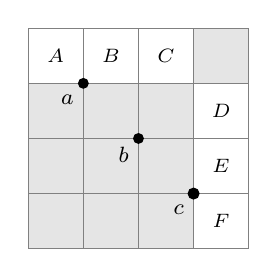
\begin{tikzpicture}[scale=0.7]

\tikzset{      
   grid/.style={        
      draw,        
      step=1cm,        
      gray!100,    
      thin,        
    },   
    cell/.style={      
      draw,      
      anchor=center,    
      text centered,    
     },    
    graycell/.style={   
      fill=gray!20,
      draw=none,     
      minimum width=1cm,   
      minimum height=1cm,     
      anchor=south west,            
    }    
  } 
    \fill[graycell] (0,0) rectangle (3,3);
  \fill[graycell] (3,3) rectangle (4,4);
 
 \draw[grid] (0,0) grid (4,4);  
 
  \node at (0.5,3.5) {\scriptsize$A$};  
  \node at (1.5,3.5) {\scriptsize$B$};  
  \node at (2.5,3.5) {\scriptsize$C$};  
  \node at (3.5,2.5) {\scriptsize$D$};
  \node at (3.5,1.5) {\scriptsize$E$};
  \node at (3.5,0.5) {\scriptsize$F$};
  \node[anchor=east] at (3,0.7) {\footnotesize{$c$}}; 
  \node[anchor=east] at (2,1.7) {\footnotesize{$b$}}; 
  \node[anchor=east] at (1,2.7) {\footnotesize{$a$}}; 
 
  \filldraw[black] (1,3) circle (2.5pt);
   \filldraw[black] (2,2) circle (2.5pt);
   \filldraw[thick] (3,1) circle (2.5pt);

\end{tikzpicture} 
	& \ & 
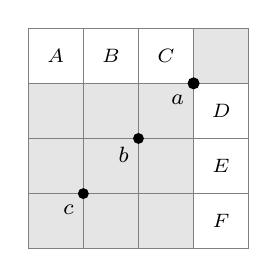
\begin{tikzpicture}[scale=0.7]

\tikzset{      
   grid/.style={        
      draw,        
      step=1cm,        
      gray!100,    
      thin,        
    },   
    cell/.style={      
      draw,      
      anchor=center,    
      text centered,    
     },    
    graycell/.style={   
      fill=gray!20,
      draw=none,     
      minimum width=1cm,   
      minimum height=1cm,     
      anchor=south west,            
    }    
  } 
      
  \fill[graycell] (0,0) rectangle (3,3);
  \fill[graycell] (3,3) rectangle (4,4);
 
 \draw[grid] (0,0) grid (4,4);  

  \node at (0.5,3.5) {\scriptsize$A$};  
  \node at (1.5,3.5) {\scriptsize$B$};  
  \node at (2.5,3.5) {\scriptsize$C$};  
  \node at (3.5,2.5) {\scriptsize$D$};
  \node at (3.5,1.5) {\scriptsize$E$};
  \node at (3.5,0.5) {\scriptsize$F$};
  \node[anchor=east] at (1,0.7) {\footnotesize{$c$}}; 
  \node[anchor=east] at (2,1.7) {\footnotesize{$b$}}; 
  \node[anchor=east] at (3,2.7) {\footnotesize{$a
  $}}; 
 
  \filldraw[black] (1,1) circle (2.5pt);
   \filldraw[black] (2,2) circle (2.5pt);
   \filldraw[thick] (3,3) circle (2.5pt);
\end{tikzpicture} 
 \end{tabular}
\vspace{-0.5cm}

\end{center}
\caption{The swapping operation that maps $\pi^{(i)}$ with the lexicographically first occurrence of $q_2$  (on the left side) to $\pi^{(i+1)}$ with one occurrence of $q_1$ (on the right side) in Theorem \ref{thm-pairs-21-22}.}\label{fig-pair21}
\end{figure}

\textbf{$f$ is well-defined.} 
% We first claim $f(\pi) \in S_n(q_2)$. 
We shall prove the sequence described above terminates in finite steps.
Let $abc$ be the lexicographically first occurrence of $q_2$ in $\pi^{(i)}$ as shown on the left side of Fig.~\ref{fig-pair21}.
We claim that no new occurrence of $q_2$ is created in $\pi^{(i+1)}$ that is lexicographically smaller than the occurrence $abc$.
Suppose, contrary to our claim, that  $a'b'c'$ is such an occurrence of $q_2$ in $\pi^{(i+1)}$. Neither a nor b can appear in $a'b'c'$, since otherwise $a'b'c'$ would not be an occurrence of $q_2$ due to the existence of $c$. 
\begin{itemize}
    \item If $c=a'$, then $b'$ and $c'$  appear in the  area $F$, which would force $cb'c'$ to be the right of $abc$, contrary to the assumption that $cb'c'$ is lexicographically smaller than the occurrence $abc$.
    \item  If $c=b'$, then $a'$ must be in area $A$ and $c'$ must be in area $F$. Therefore, $a'cc'$ would not be an occurrence of $q_2$ since $a$ and $b$ are in shaded areas.
    \item  If $c = c'$, then the elements $a'$ and $b'$ are in the area~$A$.
In this case, $a'b'a$ would be an occurrence of $q_2$ to the left of $abc$ in $\pi^{(i)}$, which is a contradiction.
\end{itemize}
This proves our claim. Thus $f(\pi)=\pi^{(j)} \in S_n(q_2)$. 

\textbf{$f$ is reversible.} We consider the inverse mapping $f^{-1}$. For any $\sigma \in S_n(q_1) \cap S_n(q_2)$, we let $f^{-1}(\sigma)=\sigma$. For $\sigma\in S_n(q_2)$ that contains occurrences of $q_1$, find the lexicographically first $q_1$ and swap the first and third elements of it. Along similar lines, we can see that the procedure never creates any new occurrences of $q_1$ that are lexicographically smaller than the lexicographically first one. 
\end{proof}

\end{document}
